\documentclass[1p]{elsarticle_modified}
%\bibliographystyle{elsarticle-num}

%\usepackage[colorlinks]{hyperref}
%\usepackage{abbrmath_seonhwa} %\Abb, \Ascr, \Acal ,\Abf, \Afrak
\usepackage{amsfonts}
\usepackage{amssymb}
\usepackage{amsmath}
\usepackage{amsthm}
\usepackage{scalefnt}
\usepackage{amsbsy}
\usepackage{kotex}
\usepackage{caption}
\usepackage{subfig}
\usepackage{color}
\usepackage{graphicx}
\usepackage{xcolor} %% white, black, red, green, blue, cyan, magenta, yellow
\usepackage{float}
\usepackage{setspace}
\usepackage{hyperref}

\usepackage{tikz}
\usetikzlibrary{arrows}

\usepackage{multirow}
\usepackage{array} % fixed length table
\usepackage{hhline}

%%%%%%%%%%%%%%%%%%%%%
\makeatletter
\renewcommand*\env@matrix[1][\arraystretch]{%
	\edef\arraystretch{#1}%
	\hskip -\arraycolsep
	\let\@ifnextchar\new@ifnextchar
	\array{*\c@MaxMatrixCols c}}
\makeatother %https://tex.stackexchange.com/questions/14071/how-can-i-increase-the-line-spacing-in-a-matrix
%%%%%%%%%%%%%%%

\usepackage[normalem]{ulem}

\newcommand{\msout}[1]{\ifmmode\text{\sout{\ensuremath{#1}}}\else\sout{#1}\fi}
%SOURCE: \msout is \stkout macro in https://tex.stackexchange.com/questions/20609/strikeout-in-math-mode

\newcommand{\cancel}[1]{
	\ifmmode
	{\color{red}\msout{#1}}
	\else
	{\color{red}\sout{#1}}
	\fi
}

\newcommand{\add}[1]{
	{\color{blue}\uwave{#1}}
}

\newcommand{\replace}[2]{
	\ifmmode
	{\color{red}\msout{#1}}{\color{blue}\uwave{#2}}
	\else
	{\color{red}\sout{#1}}{\color{blue}\uwave{#2}}
	\fi
}

\newcommand{\Sol}{\mathcal{S}} %segment
\newcommand{\D}{D} %diagram
\newcommand{\A}{\mathcal{A}} %arc


%%%%%%%%%%%%%%%%%%%%%%%%%%%%%5 test

\def\sl{\operatorname{\textup{SL}}(2,\Cbb)}
\def\psl{\operatorname{\textup{PSL}}(2,\Cbb)}
\def\quan{\mkern 1mu \triangleright \mkern 1mu}

\theoremstyle{definition}
\newtheorem{thm}{Theorem}[section]
\newtheorem{prop}[thm]{Proposition}
\newtheorem{lem}[thm]{Lemma}
\newtheorem{ques}[thm]{Question}
\newtheorem{cor}[thm]{Corollary}
\newtheorem{defn}[thm]{Definition}
\newtheorem{exam}[thm]{Example}
\newtheorem{rmk}[thm]{Remark}
\newtheorem{alg}[thm]{Algorithm}

\newcommand{\I}{\sqrt{-1}}
\begin{document}

%\begin{frontmatter}
%
%\title{Boundary parabolic representations of knots up to 8 crossings}
%
%%% Group authors per affiliation:
%\author{Yunhi Cho} 
%\address{Department of Mathematics, University of Seoul, Seoul, Korea}
%\ead{yhcho@uos.ac.kr}
%
%
%\author{Seonhwa Kim} %\fnref{s_kim}}
%\address{Center for Geometry and Physics, Institute for Basic Science, Pohang, 37673, Korea}
%\ead{ryeona17@ibs.re.kr}
%
%\author{Hyuk Kim}
%\address{Department of Mathematical Sciences, Seoul National University, Seoul 08826, Korea}
%\ead{hyukkim@snu.ac.kr}
%
%\author{Seokbeom Yoon}
%\address{Department of Mathematical Sciences, Seoul National University, Seoul, 08826,  Korea}
%\ead{sbyoon15@snu.ac.kr}
%
%\begin{abstract}
%We find all boundary parabolic representation of knots up to 8 crossings.
%
%\end{abstract}
%\begin{keyword}
%    \MSC[2010] 57M25 
%\end{keyword}
%
%\end{frontmatter}

%\linenumbers
%\tableofcontents
%
\newcommand\colored[1]{\textcolor{white}{\rule[-0.35ex]{0.8em}{1.4ex}}\kern-0.8em\color{red} #1}%
%\newcommand\colored[1]{\textcolor{white}{ #1}\kern-2.17ex	\textcolor{white}{ #1}\kern-1.81ex	\textcolor{white}{ #1}\kern-2.15ex\color{red}#1	}

{\Large $\underline{11a_{263}~(K11a_{263})}$}

\setlength{\tabcolsep}{10pt}
\renewcommand{\arraystretch}{1.6}
\vspace{1cm}\begin{tabular}{m{100pt}>{\centering\arraybackslash}m{274pt}}
\multirow{5}{120pt}{
	\centering
	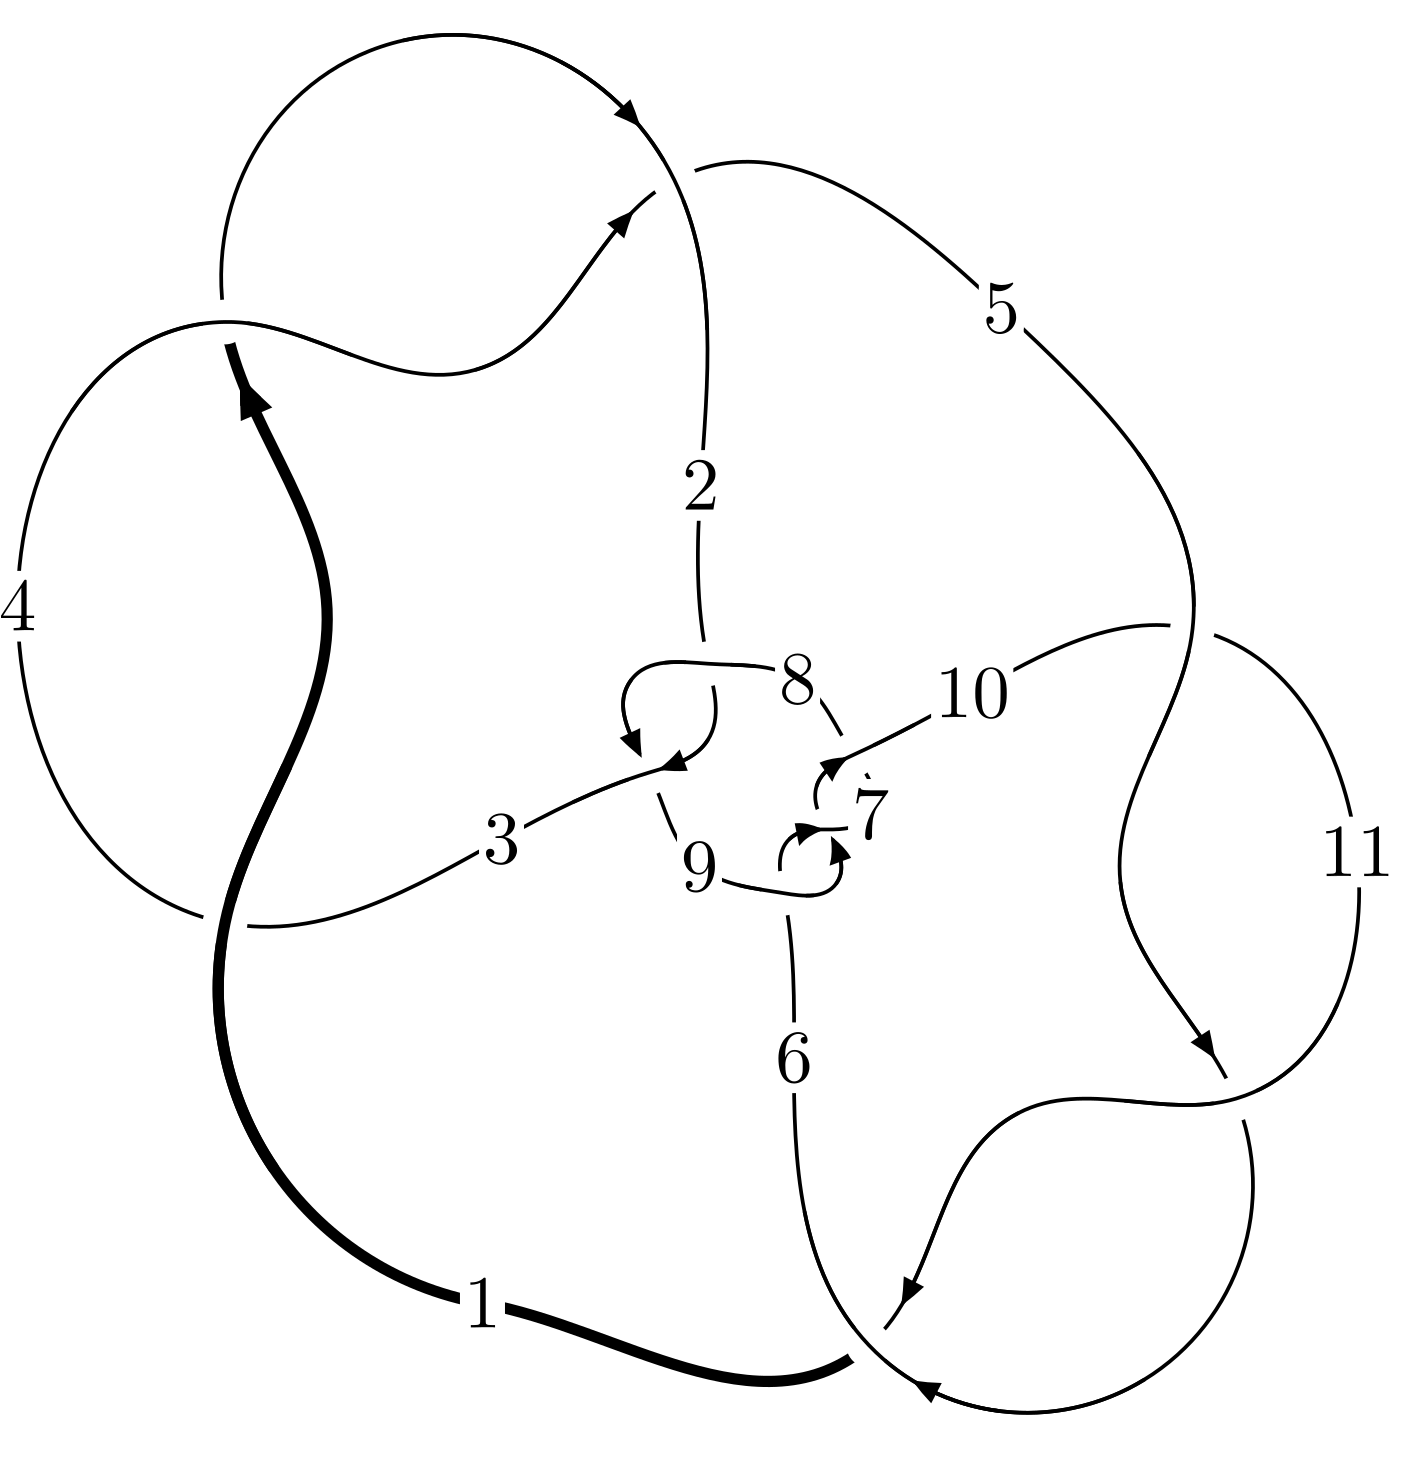
\includegraphics[width=112pt]{../../../GIT/diagram.site/Diagrams/png/512_11a_263.png}\\
\ \ \ A knot diagram\footnotemark}&
\allowdisplaybreaks
\textbf{Linearized knot diagam} \\
\cline{2-2}
 &
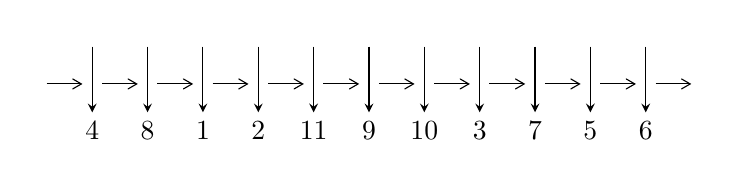
\begin{tikzpicture}[x=20pt, y=17pt]
	% nodes
	\node (C0) at (0, 0) {};
	\node (C1) at (1, 0) {};
	\node (C1U) at (1, +1) {};
	\node (C1D) at (1, -1) {4};

	\node (C2) at (2, 0) {};
	\node (C2U) at (2, +1) {};
	\node (C2D) at (2, -1) {8};

	\node (C3) at (3, 0) {};
	\node (C3U) at (3, +1) {};
	\node (C3D) at (3, -1) {1};

	\node (C4) at (4, 0) {};
	\node (C4U) at (4, +1) {};
	\node (C4D) at (4, -1) {2};

	\node (C5) at (5, 0) {};
	\node (C5U) at (5, +1) {};
	\node (C5D) at (5, -1) {11};

	\node (C6) at (6, 0) {};
	\node (C6U) at (6, +1) {};
	\node (C6D) at (6, -1) {9};

	\node (C7) at (7, 0) {};
	\node (C7U) at (7, +1) {};
	\node (C7D) at (7, -1) {10};

	\node (C8) at (8, 0) {};
	\node (C8U) at (8, +1) {};
	\node (C8D) at (8, -1) {3};

	\node (C9) at (9, 0) {};
	\node (C9U) at (9, +1) {};
	\node (C9D) at (9, -1) {7};

	\node (C10) at (10, 0) {};
	\node (C10U) at (10, +1) {};
	\node (C10D) at (10, -1) {5};

	\node (C11) at (11, 0) {};
	\node (C11U) at (11, +1) {};
	\node (C11D) at (11, -1) {6};
	\node (C12) at (12, 0) {};

	% arrows
	\draw[->,>={angle 60}]
	(C0) edge (C1) (C1) edge (C2) (C2) edge (C3) (C3) edge (C4) (C4) edge (C5) (C5) edge (C6) (C6) edge (C7) (C7) edge (C8) (C8) edge (C9) (C9) edge (C10) (C10) edge (C11) (C11) edge (C12) ;	\draw[->,>=stealth]
	(C1U) edge (C1D) (C2U) edge (C2D) (C3U) edge (C3D) (C4U) edge (C4D) (C5U) edge (C5D) (C6U) edge (C6D) (C7U) edge (C7D) (C8U) edge (C8D) (C9U) edge (C9D) (C10U) edge (C10D) (C11U) edge (C11D) ;
	\end{tikzpicture} \\
\hhline{~~} \\& 
\textbf{Solving Sequence} \\ \cline{2-2} 
 &
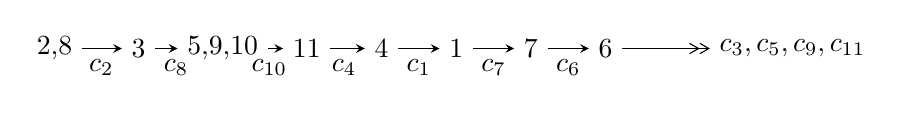
\begin{tikzpicture}[x=27pt, y=7pt]
	% node
	\node (A0) at (-1/8, 0) {2,8};
	\node (A1) at (1, 0) {3};
	\node (A2) at (17/8, 0) {5,9,10};
	\node (A3) at (13/4, 0) {11};
	\node (A4) at (17/4, 0) {4};
	\node (A5) at (21/4, 0) {1};
	\node (A6) at (25/4, 0) {7};
	\node (A7) at (29/4, 0) {6};
	\node (C1) at (1/2, -1) {$c_{2}$};
	\node (C2) at (3/2, -1) {$c_{8}$};
	\node (C3) at (11/4, -1) {$c_{10}$};
	\node (C4) at (15/4, -1) {$c_{4}$};
	\node (C5) at (19/4, -1) {$c_{1}$};
	\node (C6) at (23/4, -1) {$c_{7}$};
	\node (C7) at (27/4, -1) {$c_{6}$};
	\node (A8) at (39/4, 0) {$c_{3},c_{5},c_{9},c_{11}$};

	% edge
	\draw[->,>=stealth]	
	(A0) edge (A1) (A1) edge (A2) (A2) edge (A3) (A3) edge (A4) (A4) edge (A5) (A5) edge (A6) (A6) edge (A7) ;
	\draw[->>,>={angle 60}]	
	(A7) edge (A8);
\end{tikzpicture} \\ 

\end{tabular} \\

\footnotetext{
The image of knot diagram is generated by the software ``\textbf{Draw programme}" developed by Andrew Bartholomew(\url{http://www.layer8.co.uk/maths/draw/index.htm\#Running-draw}), where we modified some parts for our purpose(\url{https://github.com/CATsTAILs/LinksPainter}).
}\phantom \\ \newline 
\centering \textbf{Ideals for irreducible components\footnotemark of $X_{\text{par}}$} 
 
\begin{align*}
I^u_{1}&=\langle 
-9 u^7+12 u^6+5 u^5-62 u^4+26 u^3-24 u^2+92 d-64 u+16,\\
\phantom{I^u_{1}}&\phantom{= \langle  }5 u^7+u^6-13 u^5+37 u^4+6 u^3-48 u^2+92 c+56 u+32,\\
\phantom{I^u_{1}}&\phantom{= \langle  }-3 u^7+4 u^6-6 u^5-13 u^4+24 u^3-8 u^2+46 b-6 u-10,\\
\phantom{I^u_{1}}&\phantom{= \langle  }4 u^7-13 u^6+8 u^5+25 u^4-78 u^3+26 u^2+92 a+8 u-48,\;u^8- u^7- u^6+5 u^5-4 u^4+8 u^2+4 u-4\rangle \\
I^u_{2}&=\langle 
-2 u^{10}+3 u^9+2 u^8-2 u^7-2 u^6- u^5-10 u^4+21 u^3-16 u^2+4 d+10 u,\\
\phantom{I^u_{2}}&\phantom{= \langle  }- u^7+2 u^5+u^4- u^3- u^2+2 c-4 u+2,\\
\phantom{I^u_{2}}&\phantom{= \langle  }-2 u^{10}+2 u^9+3 u^8-2 u^7-2 u^6+2 u^5-9 u^4+12 u^3-7 u^2+4 b+2,\\
\phantom{I^u_{2}}&\phantom{= \langle  }2 u^{10}-3 u^9-3 u^8+4 u^7+2 u^6-3 u^5+9 u^4-15 u^3+11 u^2+4 a-6,\\
\phantom{I^u_{2}}&\phantom{= \langle  }u^{11}-2 u^{10}- u^9+3 u^8+u^7-2 u^6+4 u^5-11 u^4+9 u^3- u^2-2 u+2\rangle \\
I^u_{3}&=\langle 
u^{10}- u^9-2 u^8+u^6+u^5+7 u^4-7 u^3+2 u^2+4 d-2 u-4,\;u^{10}-3 u^8+3 u^6+2 u^4-2 u^3-3 u^2+4 c+6 u-2,\\
\phantom{I^u_{3}}&\phantom{= \langle  }u^8-2 u^6- u^5+u^4+u^3+4 u^2+2 b-2 u,\\
\phantom{I^u_{3}}&\phantom{= \langle  }-2 u^9+3 u^8+2 u^7-2 u^6-2 u^5- u^4-10 u^3+21 u^2+4 a-16 u+10,\\
\phantom{I^u_{3}}&\phantom{= \langle  }u^{11}-2 u^{10}- u^9+3 u^8+u^7-2 u^6+4 u^5-11 u^4+9 u^3- u^2-2 u+2\rangle \\
I^u_{4}&=\langle 
u^{10}- u^9-2 u^8+u^6+u^5+7 u^4-7 u^3+2 u^2+4 d-2 u-4,\;u^{10}-3 u^8+3 u^6+2 u^4-2 u^3-3 u^2+4 c+6 u-2,\\
\phantom{I^u_{4}}&\phantom{= \langle  }-2 u^{10}+2 u^9+3 u^8-2 u^7-2 u^6+2 u^5-9 u^4+12 u^3-7 u^2+4 b+2,\\
\phantom{I^u_{4}}&\phantom{= \langle  }2 u^{10}-3 u^9-3 u^8+4 u^7+2 u^6-3 u^5+9 u^4-15 u^3+11 u^2+4 a-6,\\
\phantom{I^u_{4}}&\phantom{= \langle  }u^{11}-2 u^{10}- u^9+3 u^8+u^7-2 u^6+4 u^5-11 u^4+9 u^3- u^2-2 u+2\rangle \\
I^u_{5}&=\langle 
- a^2 c- c a+d- a-1,\;- a^2 c+c^2- c a- a-1,\;a^2+b+a,\;a^3+2 a^2+a+1,\;u+1\rangle \\
\\
I^v_{1}&=\langle 
a,\;d,\;c+1,\;b-1,\;v+1\rangle \\
I^v_{2}&=\langle 
c,\;d+1,\;b,\;a-1,\;v+1\rangle \\
I^v_{3}&=\langle 
a,\;d+1,\;c+a,\;b-1,\;v+1\rangle \\
I^v_{4}&=\langle 
a,\;d a- c+1,\;d v-1,\;c v- a- v,\;b-1\rangle \\
\end{align*}
\raggedright * 8 irreducible components of $\dim_{\mathbb{C}}=0$, with total 50 representations.\\
\raggedright * 1 irreducible components of $\dim_{\mathbb{C}}=1$ \\
\footnotetext{All coefficients of polynomials are rational numbers. But the coefficients are sometimes approximated in decimal forms when there is not enough margin.}
\newpage
\renewcommand{\arraystretch}{1}
\centering \section*{I. $I^u_{1}= \langle -9 u^7+12 u^6+\cdots+92 d+16,\;5 u^7+u^6+\cdots+92 c+32,\;-3 u^7+4 u^6+\cdots+46 b-10,\;4 u^7-13 u^6+\cdots+92 a-48,\;u^8- u^7+\cdots+4 u-4 \rangle$}
\flushleft \textbf{(i) Arc colorings}\\
\begin{tabular}{m{7pt} m{180pt} m{7pt} m{180pt} }
\flushright $a_{2}=$&$\begin{pmatrix}1\\0\end{pmatrix}$ \\
\flushright $a_{8}=$&$\begin{pmatrix}0\\u\end{pmatrix}$ \\
\flushright $a_{3}=$&$\begin{pmatrix}1\\u^2\end{pmatrix}$ \\
\flushright $a_{5}=$&$\begin{pmatrix}-0.0434783 u^{7}+0.141304 u^{6}+\cdots-0.0869565 u+0.521739\\0.0652174 u^{7}-0.0869565 u^{6}+\cdots+0.130435 u+0.217391\end{pmatrix}$ \\
\flushright $a_{9}=$&$\begin{pmatrix}- u\\- u^3+u\end{pmatrix}$ \\
\flushright $a_{10}=$&$\begin{pmatrix}-0.0543478 u^{7}-0.0108696 u^{6}+\cdots-0.608696 u-0.347826\\0.0978261 u^{7}-0.130435 u^{6}+\cdots+0.695652 u-0.173913\end{pmatrix}$ \\
\flushright $a_{11}=$&$\begin{pmatrix}-0.108696 u^{7}-0.0217391 u^{6}+\cdots-0.217391 u-0.695652\\0.173913 u^{7}-0.0652174 u^{6}+\cdots+0.347826 u-0.0869565\end{pmatrix}$ \\
\flushright $a_{4}=$&$\begin{pmatrix}0.0217391 u^{7}+0.0543478 u^{6}+\cdots+0.0434783 u+0.739130\\0.0652174 u^{7}-0.0869565 u^{6}+\cdots+0.130435 u+0.217391\end{pmatrix}$ \\
\flushright $a_{1}=$&$\begin{pmatrix}0.0217391 u^{7}+0.0543478 u^{6}+\cdots+0.0434783 u+0.739130\\0.0760870 u^{7}+0.0652174 u^{6}+\cdots-0.347826 u+0.0869565\end{pmatrix}$ \\
\flushright $a_{7}=$&$\begin{pmatrix}-0.0217391 u^{7}-0.0543478 u^{6}+\cdots-0.0434783 u+0.260870\\-0.0652174 u^{7}+0.0869565 u^{6}+\cdots+0.869565 u-0.217391\end{pmatrix}$ \\
\flushright $a_{6}=$&$\begin{pmatrix}-0.0434783 u^{7}+0.141304 u^{6}+\cdots-0.0869565 u+0.521739\\0.0652174 u^{7}-0.0869565 u^{6}+\cdots+0.130435 u+0.217391\end{pmatrix}$\\ \flushright $a_{6}=$&$\begin{pmatrix}-0.0434783 u^{7}+0.141304 u^{6}+\cdots-0.0869565 u+0.521739\\0.0652174 u^{7}-0.0869565 u^{6}+\cdots+0.130435 u+0.217391\end{pmatrix}$\\&\end{tabular}
\flushleft \textbf{(ii) Obstruction class $= -1$}\\~\\
\flushleft \textbf{(iii) Cusp Shapes $= \frac{1}{23} u^7-\frac{9}{23} u^6+\frac{25}{23} u^5-\frac{11}{23} u^4-\frac{8}{23} u^3+\frac{110}{23} u^2-\frac{136}{23} u-\frac{334}{23}$}\\~\\
\newpage\renewcommand{\arraystretch}{1}
\flushleft \textbf{(iv) u-Polynomials at the component}\newline \\
\begin{tabular}{m{50pt}|m{274pt}}
Crossings & \hspace{64pt}u-Polynomials at each crossing \\
\hline $$\begin{aligned}c_{1},c_{3},c_{4}\\c_{5},c_{6},c_{7}\\c_{9},c_{10},c_{11}\end{aligned}$$&$\begin{aligned}
&u^8- u^7-5 u^6+4 u^5+8 u^4-3 u^3-3 u^2-4 u-1
\end{aligned}$\\
\hline $$\begin{aligned}c_{2},c_{8}\end{aligned}$$&$\begin{aligned}
&u^8+u^7- u^6-5 u^5-4 u^4+8 u^2-4 u-4
\end{aligned}$\\
\hline
\end{tabular}\\~\\
\newpage\renewcommand{\arraystretch}{1}
\flushleft \textbf{(v) Riley Polynomials at the component}\newline \\
\begin{tabular}{m{50pt}|m{274pt}}
Crossings & \hspace{64pt}Riley Polynomials at each crossing \\
\hline $$\begin{aligned}c_{1},c_{3},c_{4}\\c_{5},c_{6},c_{7}\\c_{9},c_{10},c_{11}\end{aligned}$$&$\begin{aligned}
&y^8-11 y^7+49 y^6-108 y^5+108 y^4-15 y^3-31 y^2-10 y+1
\end{aligned}$\\
\hline $$\begin{aligned}c_{2},c_{8}\end{aligned}$$&$\begin{aligned}
&y^8-3 y^7+3 y^6- y^5-96 y^3+96 y^2-80 y+16
\end{aligned}$\\
\hline
\end{tabular}\\~\\
\newpage\flushleft \textbf{(vi) Complex Volumes and Cusp Shapes}
$$\begin{array}{c|c|c}  
\text{Solutions to }I^u_{1}& \I (\text{vol} + \sqrt{-1}CS) & \text{Cusp shape}\\
 \hline 
\begin{aligned}
u &= -0.763708 + 0.464906 I \\
a &= \phantom{-}0.494536 + 0.909342 I \\
b &= \phantom{-}0.186694 - 0.577706 I \\
c &= \phantom{-}0.514343 - 0.443344 I \\
d &= -0.800440 - 0.464559 I\end{aligned}
 & \phantom{-}1.02858 + 1.92389 I & -7.30727 - 5.93806 I \\ \hline\begin{aligned}
u &= -0.763708 - 0.464906 I \\
a &= \phantom{-}0.494536 - 0.909342 I \\
b &= \phantom{-}0.186694 + 0.577706 I \\
c &= \phantom{-}0.514343 + 0.443344 I \\
d &= -0.800440 + 0.464559 I\end{aligned}
 & \phantom{-}1.02858 - 1.92389 I & -7.30727 + 5.93806 I \\ \hline\begin{aligned}
u &= \phantom{-}0.50215 + 1.40047 I \\
a &= -1.123050 + 0.278329 I \\
b &= \phantom{-}1.51678 - 0.24068 I \\
c &= -0.191820 + 1.014270 I \\
d &= -0.95373 - 1.43303 I\end{aligned}
 & -13.1698 + 5.8977 I & -19.7832 - 3.0693 I \\ \hline\begin{aligned}
u &= \phantom{-}0.50215 - 1.40047 I \\
a &= -1.123050 - 0.278329 I \\
b &= \phantom{-}1.51678 + 0.24068 I \\
c &= -0.191820 - 1.014270 I \\
d &= -0.95373 + 1.43303 I\end{aligned}
 & -13.1698 - 5.8977 I & -19.7832 + 3.0693 I \\ \hline\begin{aligned}
u &= \phantom{-}0.509938\phantom{ +0.000000I} \\
a &= \phantom{-}0.497054\phantom{ +0.000000I} \\
b &= \phantom{-}0.282608\phantom{ +0.000000I} \\
c &= -0.554200\phantom{ +0.000000I} \\
d &= \phantom{-}0.253467\phantom{ +0.000000I}\end{aligned}
 & -0.633408\phantom{ +0.000000I} & -16.3410\phantom{ +0.000000I} \\ \hline\begin{aligned}
u &= \phantom{-}1.37290 + 0.82084 I \\
a &= \phantom{-}0.288086 + 1.350870 I \\
b &= -1.50879 - 0.39741 I \\
c &= \phantom{-}0.937075 - 0.270804 I \\
d &= -0.71334 + 2.09107 I\end{aligned}
 & -16.0437 - 13.7204 I & -19.7312 + 6.7283 I\\
 \hline 
 \end{array}$$\newpage$$\begin{array}{c|c|c}  
\text{Solutions to }I^u_{1}& \I (\text{vol} + \sqrt{-1}CS) & \text{Cusp shape}\\
 \hline 
\begin{aligned}
u &= \phantom{-}1.37290 - 0.82084 I \\
a &= \phantom{-}0.288086 - 1.350870 I \\
b &= -1.50879 + 0.39741 I \\
c &= \phantom{-}0.937075 + 0.270804 I \\
d &= -0.71334 - 2.09107 I\end{aligned}
 & -16.0437 + 13.7204 I & -19.7312 - 6.7283 I \\ \hline\begin{aligned}
u &= -1.73262\phantom{ +0.000000I} \\
a &= \phantom{-}0.183795\phantom{ +0.000000I} \\
b &= -1.67197\phantom{ +0.000000I} \\
c &= -0.964994\phantom{ +0.000000I} \\
d &= -0.318446\phantom{ +0.000000I}\end{aligned}
 & \phantom{-}17.5248\phantom{ +0.000000I} & -22.0160\phantom{ +0.000000I}\\
 \hline 
 \end{array}$$\newpage\newpage\renewcommand{\arraystretch}{1}
\centering \section*{II. $I^u_{2}= \langle -2 u^{10}+3 u^9+\cdots+4 d+10 u,\;- u^7+2 u^5+\cdots+2 c+2,\;-2 u^{10}+2 u^9+\cdots+4 b+2,\;2 u^{10}-3 u^9+\cdots+4 a-6,\;u^{11}-2 u^{10}+\cdots-2 u+2 \rangle$}
\flushleft \textbf{(i) Arc colorings}\\
\begin{tabular}{m{7pt} m{180pt} m{7pt} m{180pt} }
\flushright $a_{2}=$&$\begin{pmatrix}1\\0\end{pmatrix}$ \\
\flushright $a_{8}=$&$\begin{pmatrix}0\\u\end{pmatrix}$ \\
\flushright $a_{3}=$&$\begin{pmatrix}1\\u^2\end{pmatrix}$ \\
\flushright $a_{5}=$&$\begin{pmatrix}-\frac{1}{2} u^{10}+\frac{3}{4} u^9+\cdots-\frac{11}{4} u^2+\frac{3}{2}\\\frac{1}{2} u^{10}-\frac{1}{2} u^9+\cdots+\frac{7}{4} u^2-\frac{1}{2}\end{pmatrix}$ \\
\flushright $a_{9}=$&$\begin{pmatrix}- u\\- u^3+u\end{pmatrix}$ \\
\flushright $a_{10}=$&$\begin{pmatrix}\frac{1}{2} u^7- u^5+\cdots+2 u-1\\\frac{1}{2} u^{10}-\frac{3}{4} u^9+\cdots+4 u^2-\frac{5}{2} u\end{pmatrix}$ \\
\flushright $a_{11}=$&$\begin{pmatrix}\frac{1}{2} u^7- u^5+\frac{1}{2} u^3+\frac{3}{2} u-1\\\frac{1}{2} u^{10}-\frac{1}{2} u^9+\cdots+\frac{7}{2} u^2-2 u\end{pmatrix}$ \\
\flushright $a_{4}=$&$\begin{pmatrix}\frac{1}{4} u^9-\frac{1}{2} u^7+\cdots- u^2+1\\\frac{1}{2} u^{10}-\frac{1}{2} u^9+\cdots+\frac{7}{4} u^2-\frac{1}{2}\end{pmatrix}$ \\
\flushright $a_{1}=$&$\begin{pmatrix}\frac{1}{4} u^9-\frac{1}{2} u^7+\cdots- u^2+1\\\frac{1}{4} u^9-\frac{1}{2} u^7+\cdots-\frac{1}{2} u^2+\frac{1}{2} u\end{pmatrix}$ \\
\flushright $a_{7}=$&$\begin{pmatrix}-\frac{1}{2} u^{10}+\frac{5}{4} u^9+\cdots+\frac{1}{2} u+1\\u^{10}-\frac{3}{2} u^9+\cdots- u-\frac{1}{2}\end{pmatrix}$ \\
\flushright $a_{6}=$&$\begin{pmatrix}-\frac{1}{2} u^{10}+\frac{3}{4} u^9+\cdots+\frac{1}{2} u+1\\-\frac{1}{2} u^9+\frac{1}{4} u^8+\cdots-2 u+\frac{1}{2}\end{pmatrix}$\\ \flushright $a_{6}=$&$\begin{pmatrix}-\frac{1}{2} u^{10}+\frac{3}{4} u^9+\cdots+\frac{1}{2} u+1\\-\frac{1}{2} u^9+\frac{1}{4} u^8+\cdots-2 u+\frac{1}{2}\end{pmatrix}$\\&\end{tabular}
\flushleft \textbf{(ii) Obstruction class $= -1$}\\~\\
\flushleft \textbf{(iii) Cusp Shapes $= 2 u^{10}-6 u^8-2 u^7+6 u^6+4 u^5+8 u^4-8 u^3-10 u^2+8 u-16$}\\~\\
\newpage\renewcommand{\arraystretch}{1}
\flushleft \textbf{(iv) u-Polynomials at the component}\newline \\
\begin{tabular}{m{50pt}|m{274pt}}
Crossings & \hspace{64pt}u-Polynomials at each crossing \\
\hline $$\begin{aligned}c_{1},c_{3},c_{4}\\c_{5},c_{10},c_{11}\end{aligned}$$&$\begin{aligned}
&u^{11}-2 u^{10}-4 u^9+8 u^8+6 u^7-8 u^6-7 u^5-2 u^4+7 u^3+3 u^2- u+1
\end{aligned}$\\
\hline $$\begin{aligned}c_{2},c_{8}\end{aligned}$$&$\begin{aligned}
&u^{11}+2 u^{10}- u^9-3 u^8+u^7+2 u^6+4 u^5+11 u^4+9 u^3+u^2-2 u-2
\end{aligned}$\\
\hline $$\begin{aligned}c_{6},c_{7},c_{9}\end{aligned}$$&$\begin{aligned}
&u^{11}-3 u^9-2 u^8+3 u^7+4 u^6-2 u^4- u^3+3 u^2-4
\end{aligned}$\\
\hline
\end{tabular}\\~\\
\newpage\renewcommand{\arraystretch}{1}
\flushleft \textbf{(v) Riley Polynomials at the component}\newline \\
\begin{tabular}{m{50pt}|m{274pt}}
Crossings & \hspace{64pt}Riley Polynomials at each crossing \\
\hline $$\begin{aligned}c_{1},c_{3},c_{4}\\c_{5},c_{10},c_{11}\end{aligned}$$&$\begin{aligned}
&y^{11}-12 y^{10}+\cdots-5 y-1
\end{aligned}$\\
\hline $$\begin{aligned}c_{2},c_{8}\end{aligned}$$&$\begin{aligned}
&y^{11}-6 y^{10}+\cdots+8 y-4
\end{aligned}$\\
\hline $$\begin{aligned}c_{6},c_{7},c_{9}\end{aligned}$$&$\begin{aligned}
&y^{11}-6 y^{10}+\cdots+24 y-16
\end{aligned}$\\
\hline
\end{tabular}\\~\\
\newpage\flushleft \textbf{(vi) Complex Volumes and Cusp Shapes}
$$\begin{array}{c|c|c}  
\text{Solutions to }I^u_{2}& \I (\text{vol} + \sqrt{-1}CS) & \text{Cusp shape}\\
 \hline 
\begin{aligned}
u &= -0.217339 + 1.116860 I \\
a &= -0.959694 - 0.121609 I \\
b &= \phantom{-}1.379210 + 0.103381 I \\
c &= \phantom{-}0.530848 - 0.577122 I \\
d &= -2.14358 + 0.93612 I\end{aligned}
 & -6.49548 - 2.41892 I & -16.9282 + 2.8895 I \\ \hline\begin{aligned}
u &= -0.217339 - 1.116860 I \\
a &= -0.959694 + 0.121609 I \\
b &= \phantom{-}1.379210 - 0.103381 I \\
c &= \phantom{-}0.530848 + 0.577122 I \\
d &= -2.14358 - 0.93612 I\end{aligned}
 & -6.49548 + 2.41892 I & -16.9282 - 2.8895 I \\ \hline\begin{aligned}
u &= \phantom{-}1.116820 + 0.404951 I \\
a &= \phantom{-}0.142488 - 1.095710 I \\
b &= \phantom{-}0.399448 + 0.789847 I \\
c &= \phantom{-}1.146260 - 0.241815 I \\
d &= -1.31237 + 1.12740 I\end{aligned}
 & -3.96110 - 4.69742 I & -14.9188 + 5.8832 I \\ \hline\begin{aligned}
u &= \phantom{-}1.116820 - 0.404951 I \\
a &= \phantom{-}0.142488 + 1.095710 I \\
b &= \phantom{-}0.399448 - 0.789847 I \\
c &= \phantom{-}1.146260 + 0.241815 I \\
d &= -1.31237 - 1.12740 I\end{aligned}
 & -3.96110 + 4.69742 I & -14.9188 - 5.8832 I \\ \hline\begin{aligned}
u &= \phantom{-}0.323694 + 0.583510 I \\
a &= \phantom{-}1.18678 - 0.80697 I \\
b &= -0.172742 + 0.362556 I \\
c &= -0.63939 + 1.57288 I \\
d &= -0.309250 - 0.329055 I\end{aligned}
 & -1.55892 + 0.74196 I & -8.46073 - 1.11909 I \\ \hline\begin{aligned}
u &= \phantom{-}0.323694 - 0.583510 I \\
a &= \phantom{-}1.18678 + 0.80697 I \\
b &= -0.172742 - 0.362556 I \\
c &= -0.63939 - 1.57288 I \\
d &= -0.309250 + 0.329055 I\end{aligned}
 & -1.55892 - 0.74196 I & -8.46073 + 1.11909 I\\
 \hline 
 \end{array}$$\newpage$$\begin{array}{c|c|c}  
\text{Solutions to }I^u_{2}& \I (\text{vol} + \sqrt{-1}CS) & \text{Cusp shape}\\
 \hline 
\begin{aligned}
u &= \phantom{-}1.38823 + 0.36743 I \\
a &= -0.243517 + 0.779738 I \\
b &= -1.50982 - 0.17565 I \\
c &= -0.526224 + 0.695676 I \\
d &= -1.10814 + 1.10674 I\end{aligned}
 & -11.90560 - 2.58451 I & -20.1919 + 1.0166 I \\ \hline\begin{aligned}
u &= \phantom{-}1.38823 - 0.36743 I \\
a &= -0.243517 - 0.779738 I \\
b &= -1.50982 + 0.17565 I \\
c &= -0.526224 - 0.695676 I \\
d &= -1.10814 - 1.10674 I\end{aligned}
 & -11.90560 + 2.58451 I & -20.1919 - 1.0166 I \\ \hline\begin{aligned}
u &= -0.552641\phantom{ +0.000000I} \\
a &= -0.218260\phantom{ +0.000000I} \\
b &= \phantom{-}0.780044\phantom{ +0.000000I} \\
c &= -2.03993\phantom{ +0.000000I} \\
d &= \phantom{-}3.71662\phantom{ +0.000000I}\end{aligned}
 & -4.41605\phantom{ +0.000000I} & -21.4290\phantom{ +0.000000I} \\ \hline\begin{aligned}
u &= -1.33508 + 0.61220 I \\
a &= -0.016930 - 1.207730 I \\
b &= -1.48612 + 0.29515 I \\
c &= \phantom{-}0.508471 - 0.520729 I \\
d &= -0.98497 - 1.74274 I\end{aligned}
 & -10.05940 + 8.65115 I & -17.7857 - 5.5789 I \\ \hline\begin{aligned}
u &= -1.33508 - 0.61220 I \\
a &= -0.016930 + 1.207730 I \\
b &= -1.48612 - 0.29515 I \\
c &= \phantom{-}0.508471 + 0.520729 I \\
d &= -0.98497 + 1.74274 I\end{aligned}
 & -10.05940 - 8.65115 I & -17.7857 + 5.5789 I\\
 \hline 
 \end{array}$$\newpage\newpage\renewcommand{\arraystretch}{1}
\centering \section*{III. $I^u_{3}= \langle u^{10}- u^9+\cdots+4 d-4,\;u^{10}-3 u^8+\cdots+4 c-2,\;u^8-2 u^6+\cdots+2 b-2 u,\;-2 u^9+3 u^8+\cdots+4 a+10,\;u^{11}-2 u^{10}+\cdots-2 u+2 \rangle$}
\flushleft \textbf{(i) Arc colorings}\\
\begin{tabular}{m{7pt} m{180pt} m{7pt} m{180pt} }
\flushright $a_{2}=$&$\begin{pmatrix}1\\0\end{pmatrix}$ \\
\flushright $a_{8}=$&$\begin{pmatrix}0\\u\end{pmatrix}$ \\
\flushright $a_{3}=$&$\begin{pmatrix}1\\u^2\end{pmatrix}$ \\
\flushright $a_{5}=$&$\begin{pmatrix}\frac{1}{2} u^9-\frac{3}{4} u^8+\cdots+4 u-\frac{5}{2}\\-\frac{1}{2} u^8+u^6+\cdots-2 u^2+u\end{pmatrix}$ \\
\flushright $a_{9}=$&$\begin{pmatrix}- u\\- u^3+u\end{pmatrix}$ \\
\flushright $a_{10}=$&$\begin{pmatrix}-\frac{1}{4} u^{10}+\frac{3}{4} u^8+\cdots-\frac{3}{2} u+\frac{1}{2}\\-\frac{1}{4} u^{10}+\frac{1}{4} u^9+\cdots+\frac{1}{2} u+1\end{pmatrix}$ \\
\flushright $a_{11}=$&$\begin{pmatrix}-\frac{1}{2} u^9+u^8+\cdots-\frac{9}{2} u+2\\1\end{pmatrix}$ \\
\flushright $a_{4}=$&$\begin{pmatrix}\frac{1}{2} u^9-\frac{5}{4} u^8+\cdots+5 u-\frac{5}{2}\\-\frac{1}{2} u^8+u^6+\cdots-2 u^2+u\end{pmatrix}$ \\
\flushright $a_{1}=$&$\begin{pmatrix}\frac{1}{2} u^9-\frac{5}{4} u^8+\cdots+5 u-\frac{5}{2}\\-\frac{1}{4} u^{10}+\frac{1}{2} u^8+\cdots+u^3-1\end{pmatrix}$ \\
\flushright $a_{7}=$&$\begin{pmatrix}-\frac{1}{4} u^8+\frac{1}{2} u^6+\cdots+\frac{1}{2} u-\frac{1}{2}\\\frac{1}{2} u^5-\frac{1}{2} u^3-\frac{1}{2} u^2+u\end{pmatrix}$ \\
\flushright $a_{6}=$&$\begin{pmatrix}\frac{1}{2} u^{10}-\frac{1}{4} u^9+\cdots+u-\frac{3}{2}\\\frac{1}{2} u^{10}-\frac{1}{2} u^9+\cdots+u-\frac{1}{2}\end{pmatrix}$\\ \flushright $a_{6}=$&$\begin{pmatrix}\frac{1}{2} u^{10}-\frac{1}{4} u^9+\cdots+u-\frac{3}{2}\\\frac{1}{2} u^{10}-\frac{1}{2} u^9+\cdots+u-\frac{1}{2}\end{pmatrix}$\\&\end{tabular}
\flushleft \textbf{(ii) Obstruction class $= -1$}\\~\\
\flushleft \textbf{(iii) Cusp Shapes $= 2 u^{10}-6 u^8-2 u^7+6 u^6+4 u^5+8 u^4-8 u^3-10 u^2+8 u-16$}\\~\\
\newpage\renewcommand{\arraystretch}{1}
\flushleft \textbf{(iv) u-Polynomials at the component}\newline \\
\begin{tabular}{m{50pt}|m{274pt}}
Crossings & \hspace{64pt}u-Polynomials at each crossing \\
\hline $$\begin{aligned}c_{1},c_{3},c_{4}\end{aligned}$$&$\begin{aligned}
&u^{11}-3 u^9-2 u^8+3 u^7+4 u^6-2 u^4- u^3+3 u^2-4
\end{aligned}$\\
\hline $$\begin{aligned}c_{2},c_{8}\end{aligned}$$&$\begin{aligned}
&u^{11}+2 u^{10}- u^9-3 u^8+u^7+2 u^6+4 u^5+11 u^4+9 u^3+u^2-2 u-2
\end{aligned}$\\
\hline $$\begin{aligned}c_{5},c_{6},c_{7}\\c_{9},c_{10},c_{11}\end{aligned}$$&$\begin{aligned}
&u^{11}-2 u^{10}-4 u^9+8 u^8+6 u^7-8 u^6-7 u^5-2 u^4+7 u^3+3 u^2- u+1
\end{aligned}$\\
\hline
\end{tabular}\\~\\
\newpage\renewcommand{\arraystretch}{1}
\flushleft \textbf{(v) Riley Polynomials at the component}\newline \\
\begin{tabular}{m{50pt}|m{274pt}}
Crossings & \hspace{64pt}Riley Polynomials at each crossing \\
\hline $$\begin{aligned}c_{1},c_{3},c_{4}\end{aligned}$$&$\begin{aligned}
&y^{11}-6 y^{10}+\cdots+24 y-16
\end{aligned}$\\
\hline $$\begin{aligned}c_{2},c_{8}\end{aligned}$$&$\begin{aligned}
&y^{11}-6 y^{10}+\cdots+8 y-4
\end{aligned}$\\
\hline $$\begin{aligned}c_{5},c_{6},c_{7}\\c_{9},c_{10},c_{11}\end{aligned}$$&$\begin{aligned}
&y^{11}-12 y^{10}+\cdots-5 y-1
\end{aligned}$\\
\hline
\end{tabular}\\~\\
\newpage\flushleft \textbf{(vi) Complex Volumes and Cusp Shapes}
$$\begin{array}{c|c|c}  
\text{Solutions to }I^u_{3}& \I (\text{vol} + \sqrt{-1}CS) & \text{Cusp shape}\\
 \hline 
\begin{aligned}
u &= -0.217339 + 1.116860 I \\
a &= \phantom{-}1.16746 + 1.69211 I \\
b &= -0.529187 - 0.718311 I \\
c &= \phantom{-}0.142356 + 1.207200 I \\
d &= \phantom{-}0.344399 - 1.045410 I\end{aligned}
 & -6.49548 - 2.41892 I & -16.9282 + 2.8895 I \\ \hline\begin{aligned}
u &= -0.217339 - 1.116860 I \\
a &= \phantom{-}1.16746 - 1.69211 I \\
b &= -0.529187 + 0.718311 I \\
c &= \phantom{-}0.142356 - 1.207200 I \\
d &= \phantom{-}0.344399 + 1.045410 I\end{aligned}
 & -6.49548 + 2.41892 I & -16.9282 - 2.8895 I \\ \hline\begin{aligned}
u &= \phantom{-}1.116820 + 0.404951 I \\
a &= -0.71505 + 1.26875 I \\
b &= -1.378090 - 0.194114 I \\
c &= -0.542743 - 0.510432 I \\
d &= \phantom{-}0.602844 - 1.166020 I\end{aligned}
 & -3.96110 - 4.69742 I & -14.9188 + 5.8832 I \\ \hline\begin{aligned}
u &= \phantom{-}1.116820 - 0.404951 I \\
a &= -0.71505 - 1.26875 I \\
b &= -1.378090 + 0.194114 I \\
c &= -0.542743 + 0.510432 I \\
d &= \phantom{-}0.602844 + 1.166020 I\end{aligned}
 & -3.96110 + 4.69742 I & -14.9188 - 5.8832 I \\ \hline\begin{aligned}
u &= \phantom{-}0.323694 + 0.583510 I \\
a &= -0.656040 + 0.166054 I \\
b &= \phantom{-}1.124760 - 0.136043 I \\
c &= -0.349546 - 0.489945 I \\
d &= \phantom{-}0.855030 + 0.431288 I\end{aligned}
 & -1.55892 + 0.74196 I & -8.46073 - 1.11909 I \\ \hline\begin{aligned}
u &= \phantom{-}0.323694 - 0.583510 I \\
a &= -0.656040 - 0.166054 I \\
b &= \phantom{-}1.124760 + 0.136043 I \\
c &= -0.349546 + 0.489945 I \\
d &= \phantom{-}0.855030 - 0.431288 I\end{aligned}
 & -1.55892 - 0.74196 I & -8.46073 + 1.11909 I\\
 \hline 
 \end{array}$$\newpage$$\begin{array}{c|c|c}  
\text{Solutions to }I^u_{3}& \I (\text{vol} + \sqrt{-1}CS) & \text{Cusp shape}\\
 \hline 
\begin{aligned}
u &= \phantom{-}1.38823 + 0.36743 I \\
a &= -0.548785 + 0.942487 I \\
b &= \phantom{-}0.986131 - 0.772404 I \\
c &= \phantom{-}1.047690 - 0.150769 I \\
d &= -0.624556 + 0.992977 I\end{aligned}
 & -11.90560 - 2.58451 I & -20.1919 + 1.0166 I \\ \hline\begin{aligned}
u &= \phantom{-}1.38823 - 0.36743 I \\
a &= -0.548785 - 0.942487 I \\
b &= \phantom{-}0.986131 + 0.772404 I \\
c &= \phantom{-}1.047690 + 0.150769 I \\
d &= -0.624556 - 0.992977 I\end{aligned}
 & -11.90560 + 2.58451 I & -20.1919 - 1.0166 I \\ \hline\begin{aligned}
u &= -0.552641\phantom{ +0.000000I} \\
a &= -6.72520\phantom{ +0.000000I} \\
b &= -1.12735\phantom{ +0.000000I} \\
c &= \phantom{-}1.41149\phantom{ +0.000000I} \\
d &= \phantom{-}0.120619\phantom{ +0.000000I}\end{aligned}
 & -4.41605\phantom{ +0.000000I} & -21.4290\phantom{ +0.000000I} \\ \hline\begin{aligned}
u &= -1.33508 + 0.61220 I \\
a &= \phantom{-}0.115017 + 1.358080 I \\
b &= \phantom{-}0.360061 - 1.006500 I \\
c &= -1.003500 - 0.239081 I \\
d &= \phantom{-}0.76197 + 1.60205 I\end{aligned}
 & -10.05940 + 8.65115 I & -17.7857 - 5.5789 I \\ \hline\begin{aligned}
u &= -1.33508 - 0.61220 I \\
a &= \phantom{-}0.115017 - 1.358080 I \\
b &= \phantom{-}0.360061 + 1.006500 I \\
c &= -1.003500 + 0.239081 I \\
d &= \phantom{-}0.76197 - 1.60205 I\end{aligned}
 & -10.05940 - 8.65115 I & -17.7857 + 5.5789 I\\
 \hline 
 \end{array}$$\newpage\newpage\renewcommand{\arraystretch}{1}
\centering \section*{IV. $I^u_{4}= \langle u^{10}- u^9+\cdots+4 d-4,\;u^{10}-3 u^8+\cdots+4 c-2,\;-2 u^{10}+2 u^9+\cdots+4 b+2,\;2 u^{10}-3 u^9+\cdots+4 a-6,\;u^{11}-2 u^{10}+\cdots-2 u+2 \rangle$}
\flushleft \textbf{(i) Arc colorings}\\
\begin{tabular}{m{7pt} m{180pt} m{7pt} m{180pt} }
\flushright $a_{2}=$&$\begin{pmatrix}1\\0\end{pmatrix}$ \\
\flushright $a_{8}=$&$\begin{pmatrix}0\\u\end{pmatrix}$ \\
\flushright $a_{3}=$&$\begin{pmatrix}1\\u^2\end{pmatrix}$ \\
\flushright $a_{5}=$&$\begin{pmatrix}-\frac{1}{2} u^{10}+\frac{3}{4} u^9+\cdots-\frac{11}{4} u^2+\frac{3}{2}\\\frac{1}{2} u^{10}-\frac{1}{2} u^9+\cdots+\frac{7}{4} u^2-\frac{1}{2}\end{pmatrix}$ \\
\flushright $a_{9}=$&$\begin{pmatrix}- u\\- u^3+u\end{pmatrix}$ \\
\flushright $a_{10}=$&$\begin{pmatrix}-\frac{1}{4} u^{10}+\frac{3}{4} u^8+\cdots-\frac{3}{2} u+\frac{1}{2}\\-\frac{1}{4} u^{10}+\frac{1}{4} u^9+\cdots+\frac{1}{2} u+1\end{pmatrix}$ \\
\flushright $a_{11}=$&$\begin{pmatrix}-\frac{1}{2} u^{10}+\frac{3}{2} u^8+\cdots+\frac{5}{2} u^2-\frac{3}{2} u\\1\end{pmatrix}$ \\
\flushright $a_{4}=$&$\begin{pmatrix}\frac{1}{4} u^9-\frac{1}{2} u^7+\cdots- u^2+1\\\frac{1}{2} u^{10}-\frac{1}{2} u^9+\cdots+\frac{7}{4} u^2-\frac{1}{2}\end{pmatrix}$ \\
\flushright $a_{1}=$&$\begin{pmatrix}\frac{1}{4} u^9-\frac{1}{2} u^7+\cdots- u^2+1\\\frac{1}{4} u^9-\frac{1}{2} u^7+\cdots-\frac{1}{2} u^2+\frac{1}{2} u\end{pmatrix}$ \\
\flushright $a_{7}=$&$\begin{pmatrix}-\frac{1}{4} u^8+\frac{1}{2} u^6+\cdots+\frac{1}{2} u-\frac{1}{2}\\\frac{1}{2} u^5-\frac{1}{2} u^3-\frac{1}{2} u^2+u\end{pmatrix}$ \\
\flushright $a_{6}=$&$\begin{pmatrix}\frac{1}{2} u^{10}-\frac{1}{4} u^9+\cdots+u-\frac{3}{2}\\\frac{1}{2} u^{10}-\frac{1}{2} u^9+\cdots+u-\frac{1}{2}\end{pmatrix}$\\ \flushright $a_{6}=$&$\begin{pmatrix}\frac{1}{2} u^{10}-\frac{1}{4} u^9+\cdots+u-\frac{3}{2}\\\frac{1}{2} u^{10}-\frac{1}{2} u^9+\cdots+u-\frac{1}{2}\end{pmatrix}$\\&\end{tabular}
\flushleft \textbf{(ii) Obstruction class $= -1$}\\~\\
\flushleft \textbf{(iii) Cusp Shapes $= 2 u^{10}-6 u^8-2 u^7+6 u^6+4 u^5+8 u^4-8 u^3-10 u^2+8 u-16$}\\~\\
\newpage\renewcommand{\arraystretch}{1}
\flushleft \textbf{(iv) u-Polynomials at the component}\newline \\
\begin{tabular}{m{50pt}|m{274pt}}
Crossings & \hspace{64pt}u-Polynomials at each crossing \\
\hline $$\begin{aligned}c_{1},c_{3},c_{4}\\c_{6},c_{7},c_{9}\end{aligned}$$&$\begin{aligned}
&u^{11}-2 u^{10}-4 u^9+8 u^8+6 u^7-8 u^6-7 u^5-2 u^4+7 u^3+3 u^2- u+1
\end{aligned}$\\
\hline $$\begin{aligned}c_{2},c_{8}\end{aligned}$$&$\begin{aligned}
&u^{11}+2 u^{10}- u^9-3 u^8+u^7+2 u^6+4 u^5+11 u^4+9 u^3+u^2-2 u-2
\end{aligned}$\\
\hline $$\begin{aligned}c_{5},c_{10},c_{11}\end{aligned}$$&$\begin{aligned}
&u^{11}-3 u^9-2 u^8+3 u^7+4 u^6-2 u^4- u^3+3 u^2-4
\end{aligned}$\\
\hline
\end{tabular}\\~\\
\newpage\renewcommand{\arraystretch}{1}
\flushleft \textbf{(v) Riley Polynomials at the component}\newline \\
\begin{tabular}{m{50pt}|m{274pt}}
Crossings & \hspace{64pt}Riley Polynomials at each crossing \\
\hline $$\begin{aligned}c_{1},c_{3},c_{4}\\c_{6},c_{7},c_{9}\end{aligned}$$&$\begin{aligned}
&y^{11}-12 y^{10}+\cdots-5 y-1
\end{aligned}$\\
\hline $$\begin{aligned}c_{2},c_{8}\end{aligned}$$&$\begin{aligned}
&y^{11}-6 y^{10}+\cdots+8 y-4
\end{aligned}$\\
\hline $$\begin{aligned}c_{5},c_{10},c_{11}\end{aligned}$$&$\begin{aligned}
&y^{11}-6 y^{10}+\cdots+24 y-16
\end{aligned}$\\
\hline
\end{tabular}\\~\\
\newpage\flushleft \textbf{(vi) Complex Volumes and Cusp Shapes}
$$\begin{array}{c|c|c}  
\text{Solutions to }I^u_{4}& \I (\text{vol} + \sqrt{-1}CS) & \text{Cusp shape}\\
 \hline 
\begin{aligned}
u &= -0.217339 + 1.116860 I \\
a &= -0.959694 - 0.121609 I \\
b &= \phantom{-}1.379210 + 0.103381 I \\
c &= \phantom{-}0.142356 + 1.207200 I \\
d &= \phantom{-}0.344399 - 1.045410 I\end{aligned}
 & -6.49548 - 2.41892 I & -16.9282 + 2.8895 I \\ \hline\begin{aligned}
u &= -0.217339 - 1.116860 I \\
a &= -0.959694 + 0.121609 I \\
b &= \phantom{-}1.379210 - 0.103381 I \\
c &= \phantom{-}0.142356 - 1.207200 I \\
d &= \phantom{-}0.344399 + 1.045410 I\end{aligned}
 & -6.49548 + 2.41892 I & -16.9282 - 2.8895 I \\ \hline\begin{aligned}
u &= \phantom{-}1.116820 + 0.404951 I \\
a &= \phantom{-}0.142488 - 1.095710 I \\
b &= \phantom{-}0.399448 + 0.789847 I \\
c &= -0.542743 - 0.510432 I \\
d &= \phantom{-}0.602844 - 1.166020 I\end{aligned}
 & -3.96110 - 4.69742 I & -14.9188 + 5.8832 I \\ \hline\begin{aligned}
u &= \phantom{-}1.116820 - 0.404951 I \\
a &= \phantom{-}0.142488 + 1.095710 I \\
b &= \phantom{-}0.399448 - 0.789847 I \\
c &= -0.542743 + 0.510432 I \\
d &= \phantom{-}0.602844 + 1.166020 I\end{aligned}
 & -3.96110 + 4.69742 I & -14.9188 - 5.8832 I \\ \hline\begin{aligned}
u &= \phantom{-}0.323694 + 0.583510 I \\
a &= \phantom{-}1.18678 - 0.80697 I \\
b &= -0.172742 + 0.362556 I \\
c &= -0.349546 - 0.489945 I \\
d &= \phantom{-}0.855030 + 0.431288 I\end{aligned}
 & -1.55892 + 0.74196 I & -8.46073 - 1.11909 I \\ \hline\begin{aligned}
u &= \phantom{-}0.323694 - 0.583510 I \\
a &= \phantom{-}1.18678 + 0.80697 I \\
b &= -0.172742 - 0.362556 I \\
c &= -0.349546 + 0.489945 I \\
d &= \phantom{-}0.855030 - 0.431288 I\end{aligned}
 & -1.55892 - 0.74196 I & -8.46073 + 1.11909 I\\
 \hline 
 \end{array}$$\newpage$$\begin{array}{c|c|c}  
\text{Solutions to }I^u_{4}& \I (\text{vol} + \sqrt{-1}CS) & \text{Cusp shape}\\
 \hline 
\begin{aligned}
u &= \phantom{-}1.38823 + 0.36743 I \\
a &= -0.243517 + 0.779738 I \\
b &= -1.50982 - 0.17565 I \\
c &= \phantom{-}1.047690 - 0.150769 I \\
d &= -0.624556 + 0.992977 I\end{aligned}
 & -11.90560 - 2.58451 I & -20.1919 + 1.0166 I \\ \hline\begin{aligned}
u &= \phantom{-}1.38823 - 0.36743 I \\
a &= -0.243517 - 0.779738 I \\
b &= -1.50982 + 0.17565 I \\
c &= \phantom{-}1.047690 + 0.150769 I \\
d &= -0.624556 - 0.992977 I\end{aligned}
 & -11.90560 + 2.58451 I & -20.1919 - 1.0166 I \\ \hline\begin{aligned}
u &= -0.552641\phantom{ +0.000000I} \\
a &= -0.218260\phantom{ +0.000000I} \\
b &= \phantom{-}0.780044\phantom{ +0.000000I} \\
c &= \phantom{-}1.41149\phantom{ +0.000000I} \\
d &= \phantom{-}0.120619\phantom{ +0.000000I}\end{aligned}
 & -4.41605\phantom{ +0.000000I} & -21.4290\phantom{ +0.000000I} \\ \hline\begin{aligned}
u &= -1.33508 + 0.61220 I \\
a &= -0.016930 - 1.207730 I \\
b &= -1.48612 + 0.29515 I \\
c &= -1.003500 - 0.239081 I \\
d &= \phantom{-}0.76197 + 1.60205 I\end{aligned}
 & -10.05940 + 8.65115 I & -17.7857 - 5.5789 I \\ \hline\begin{aligned}
u &= -1.33508 - 0.61220 I \\
a &= -0.016930 + 1.207730 I \\
b &= -1.48612 - 0.29515 I \\
c &= -1.003500 + 0.239081 I \\
d &= \phantom{-}0.76197 - 1.60205 I\end{aligned}
 & -10.05940 - 8.65115 I & -17.7857 + 5.5789 I\\
 \hline 
 \end{array}$$\newpage\newpage\renewcommand{\arraystretch}{1}
\centering \section*{V. $I^u_{5}= \langle - a^2 c- c a+d- a-1,\;- a^2 c+c^2- c a- a-1,\;a^2+b+a,\;a^3+2 a^2+a+1,\;u+1 \rangle$}
\flushleft \textbf{(i) Arc colorings}\\
\begin{tabular}{m{7pt} m{180pt} m{7pt} m{180pt} }
\flushright $a_{2}=$&$\begin{pmatrix}1\\0\end{pmatrix}$ \\
\flushright $a_{8}=$&$\begin{pmatrix}0\\-1\end{pmatrix}$ \\
\flushright $a_{3}=$&$\begin{pmatrix}1\\1\end{pmatrix}$ \\
\flushright $a_{5}=$&$\begin{pmatrix}a\\- a^2- a\end{pmatrix}$ \\
\flushright $a_{9}=$&$\begin{pmatrix}1\\0\end{pmatrix}$ \\
\flushright $a_{10}=$&$\begin{pmatrix}c\\a^2 c+c a+a+1\end{pmatrix}$ \\
\flushright $a_{11}=$&$\begin{pmatrix}c a+a^2+c+a+1\\1\end{pmatrix}$ \\
\flushright $a_{4}=$&$\begin{pmatrix}- a^2\\- a^2- a\end{pmatrix}$ \\
\flushright $a_{1}=$&$\begin{pmatrix}- a^2\\a\end{pmatrix}$ \\
\flushright $a_{7}=$&$\begin{pmatrix}- a^2 c- c a- a-1\\- c\end{pmatrix}$ \\
\flushright $a_{6}=$&$\begin{pmatrix}- a^2 c- c a- c- a-1\\- c\end{pmatrix}$\\ \flushright $a_{6}=$&$\begin{pmatrix}- a^2 c- c a- c- a-1\\- c\end{pmatrix}$\\&\end{tabular}
\flushleft \textbf{(ii) Obstruction class $= -1$}\\~\\
\flushleft \textbf{(iii) Cusp Shapes $= -18$}\\~\\
\newpage\renewcommand{\arraystretch}{1}
\flushleft \textbf{(iv) u-Polynomials at the component}\newline \\
\begin{tabular}{m{50pt}|m{274pt}}
Crossings & \hspace{64pt}u-Polynomials at each crossing \\
\hline $$\begin{aligned}c_{1},c_{3},c_{4}\\c_{5},c_{6},c_{7}\\c_{9},c_{10},c_{11}\end{aligned}$$&$\begin{aligned}
&(u^3- u-1)^2
\end{aligned}$\\
\hline $$\begin{aligned}c_{2},c_{8}\end{aligned}$$&$\begin{aligned}
&(u-1)^6
\end{aligned}$\\
\hline
\end{tabular}\\~\\
\newpage\renewcommand{\arraystretch}{1}
\flushleft \textbf{(v) Riley Polynomials at the component}\newline \\
\begin{tabular}{m{50pt}|m{274pt}}
Crossings & \hspace{64pt}Riley Polynomials at each crossing \\
\hline $$\begin{aligned}c_{1},c_{3},c_{4}\\c_{5},c_{6},c_{7}\\c_{9},c_{10},c_{11}\end{aligned}$$&$\begin{aligned}
&(y^3-2 y^2+y-1)^2
\end{aligned}$\\
\hline $$\begin{aligned}c_{2},c_{8}\end{aligned}$$&$\begin{aligned}
&(y-1)^6
\end{aligned}$\\
\hline
\end{tabular}\\~\\
\newpage\flushleft \textbf{(vi) Complex Volumes and Cusp Shapes}
$$\begin{array}{c|c|c}  
\text{Solutions to }I^u_{5}& \I (\text{vol} + \sqrt{-1}CS) & \text{Cusp shape}\\
 \hline 
\begin{aligned}
u &= -1.00000\phantom{ +0.000000I} \\
a &= -0.122561 + 0.744862 I \\
b &= \phantom{-}0.662359 - 0.562280 I \\
c &= \phantom{-}0.662359 + 0.562280 I \\
d &= \phantom{-}0.122561 + 0.744862 I\end{aligned}
 & -4.93480\phantom{ +0.000000I} & -18.0000\phantom{ +0.000000I} \\ \hline\begin{aligned}
u &= -1.00000\phantom{ +0.000000I} \\
a &= -0.122561 + 0.744862 I \\
b &= \phantom{-}0.662359 - 0.562280 I \\
c &= -1.32472\phantom{ +0.000000I} \\
d &= \phantom{-}1.75488\phantom{ +0.000000I}\end{aligned}
 & -4.93480\phantom{ +0.000000I} & -18.0000\phantom{ +0.000000I} \\ \hline\begin{aligned}
u &= -1.00000\phantom{ +0.000000I} \\
a &= -0.122561 - 0.744862 I \\
b &= \phantom{-}0.662359 + 0.562280 I \\
c &= \phantom{-}0.662359 - 0.562280 I \\
d &= \phantom{-}0.122561 - 0.744862 I\end{aligned}
 & -4.93480\phantom{ +0.000000I} & -18.0000\phantom{ +0.000000I} \\ \hline\begin{aligned}
u &= -1.00000\phantom{ +0.000000I} \\
a &= -0.122561 - 0.744862 I \\
b &= \phantom{-}0.662359 + 0.562280 I \\
c &= -1.32472\phantom{ +0.000000I} \\
d &= \phantom{-}1.75488\phantom{ +0.000000I}\end{aligned}
 & -4.93480\phantom{ +0.000000I} & -18.0000\phantom{ +0.000000I} \\ \hline\begin{aligned}
u &= -1.00000\phantom{ +0.000000I} \\
a &= -1.75488\phantom{ +0.000000I} \\
b &= -1.32472\phantom{ +0.000000I} \\
c &= \phantom{-}0.662359 + 0.562280 I \\
d &= \phantom{-}0.122561 + 0.744862 I\end{aligned}
 & -4.93480\phantom{ +0.000000I} & -18.0000\phantom{ +0.000000I} \\ \hline\begin{aligned}
u &= -1.00000\phantom{ +0.000000I} \\
a &= -1.75488\phantom{ +0.000000I} \\
b &= -1.32472\phantom{ +0.000000I} \\
c &= \phantom{-}0.662359 - 0.562280 I \\
d &= \phantom{-}0.122561 - 0.744862 I\end{aligned}
 & -4.93480\phantom{ +0.000000I} & -18.0000\phantom{ +0.000000I}\\
 \hline 
 \end{array}$$\newpage\newpage\renewcommand{\arraystretch}{1}
\centering \section*{VI. $I^v_{1}= \langle a,\;d,\;c+1,\;b-1,\;v+1 \rangle$}
\flushleft \textbf{(i) Arc colorings}\\
\begin{tabular}{m{7pt} m{180pt} m{7pt} m{180pt} }
\flushright $a_{2}=$&$\begin{pmatrix}1\\0\end{pmatrix}$ \\
\flushright $a_{8}=$&$\begin{pmatrix}-1\\0\end{pmatrix}$ \\
\flushright $a_{3}=$&$\begin{pmatrix}1\\0\end{pmatrix}$ \\
\flushright $a_{5}=$&$\begin{pmatrix}0\\1\end{pmatrix}$ \\
\flushright $a_{9}=$&$\begin{pmatrix}-1\\0\end{pmatrix}$ \\
\flushright $a_{10}=$&$\begin{pmatrix}-1\\0\end{pmatrix}$ \\
\flushright $a_{11}=$&$\begin{pmatrix}-1\\-1\end{pmatrix}$ \\
\flushright $a_{4}=$&$\begin{pmatrix}1\\1\end{pmatrix}$ \\
\flushright $a_{1}=$&$\begin{pmatrix}0\\-1\end{pmatrix}$ \\
\flushright $a_{7}=$&$\begin{pmatrix}-1\\0\end{pmatrix}$ \\
\flushright $a_{6}=$&$\begin{pmatrix}-1\\0\end{pmatrix}$\\ \flushright $a_{6}=$&$\begin{pmatrix}-1\\0\end{pmatrix}$\\&\end{tabular}
\flushleft \textbf{(ii) Obstruction class $= 1$}\\~\\
\flushleft \textbf{(iii) Cusp Shapes $= -12$}\\~\\
\newpage\renewcommand{\arraystretch}{1}
\flushleft \textbf{(iv) u-Polynomials at the component}\newline \\
\begin{tabular}{m{50pt}|m{274pt}}
Crossings & \hspace{64pt}u-Polynomials at each crossing \\
\hline $$\begin{aligned}c_{1},c_{5}\end{aligned}$$&$\begin{aligned}
&u-1
\end{aligned}$\\
\hline $$\begin{aligned}c_{2},c_{6},c_{7}\\c_{8},c_{9}\end{aligned}$$&$\begin{aligned}
&u
\end{aligned}$\\
\hline $$\begin{aligned}c_{3},c_{4},c_{10}\\c_{11}\end{aligned}$$&$\begin{aligned}
&u+1
\end{aligned}$\\
\hline
\end{tabular}\\~\\
\newpage\renewcommand{\arraystretch}{1}
\flushleft \textbf{(v) Riley Polynomials at the component}\newline \\
\begin{tabular}{m{50pt}|m{274pt}}
Crossings & \hspace{64pt}Riley Polynomials at each crossing \\
\hline $$\begin{aligned}c_{1},c_{3},c_{4}\\c_{5},c_{10},c_{11}\end{aligned}$$&$\begin{aligned}
&y-1
\end{aligned}$\\
\hline $$\begin{aligned}c_{2},c_{6},c_{7}\\c_{8},c_{9}\end{aligned}$$&$\begin{aligned}
&y
\end{aligned}$\\
\hline
\end{tabular}\\~\\
\newpage\flushleft \textbf{(vi) Complex Volumes and Cusp Shapes}
$$\begin{array}{c|c|c}  
\text{Solutions to }I^v_{1}& \I (\text{vol} + \sqrt{-1}CS) & \text{Cusp shape}\\
 \hline 
\begin{aligned}
v &= -1.00000\phantom{ +0.000000I} \\
a &= \phantom{-0.000000 } 0 \\
b &= \phantom{-}1.00000\phantom{ +0.000000I} \\
c &= -1.00000\phantom{ +0.000000I} \\
d &= \phantom{-0.000000 } 0\end{aligned}
 & -3.28987\phantom{ +0.000000I} & -12.0000\phantom{ +0.000000I}\\
 \hline 
 \end{array}$$\newpage\newpage\renewcommand{\arraystretch}{1}
\centering \section*{VII. $I^v_{2}= \langle c,\;d+1,\;b,\;a-1,\;v+1 \rangle$}
\flushleft \textbf{(i) Arc colorings}\\
\begin{tabular}{m{7pt} m{180pt} m{7pt} m{180pt} }
\flushright $a_{2}=$&$\begin{pmatrix}1\\0\end{pmatrix}$ \\
\flushright $a_{8}=$&$\begin{pmatrix}-1\\0\end{pmatrix}$ \\
\flushright $a_{3}=$&$\begin{pmatrix}1\\0\end{pmatrix}$ \\
\flushright $a_{5}=$&$\begin{pmatrix}1\\0\end{pmatrix}$ \\
\flushright $a_{9}=$&$\begin{pmatrix}-1\\0\end{pmatrix}$ \\
\flushright $a_{10}=$&$\begin{pmatrix}0\\-1\end{pmatrix}$ \\
\flushright $a_{11}=$&$\begin{pmatrix}1\\-1\end{pmatrix}$ \\
\flushright $a_{4}=$&$\begin{pmatrix}1\\0\end{pmatrix}$ \\
\flushright $a_{1}=$&$\begin{pmatrix}1\\0\end{pmatrix}$ \\
\flushright $a_{7}=$&$\begin{pmatrix}-1\\1\end{pmatrix}$ \\
\flushright $a_{6}=$&$\begin{pmatrix}0\\1\end{pmatrix}$\\ \flushright $a_{6}=$&$\begin{pmatrix}0\\1\end{pmatrix}$\\&\end{tabular}
\flushleft \textbf{(ii) Obstruction class $= 1$}\\~\\
\flushleft \textbf{(iii) Cusp Shapes $= -12$}\\~\\
\newpage\renewcommand{\arraystretch}{1}
\flushleft \textbf{(iv) u-Polynomials at the component}\newline \\
\begin{tabular}{m{50pt}|m{274pt}}
Crossings & \hspace{64pt}u-Polynomials at each crossing \\
\hline $$\begin{aligned}c_{1},c_{2},c_{3}\\c_{4},c_{8}\end{aligned}$$&$\begin{aligned}
&u
\end{aligned}$\\
\hline $$\begin{aligned}c_{5},c_{9}\end{aligned}$$&$\begin{aligned}
&u+1
\end{aligned}$\\
\hline $$\begin{aligned}c_{6},c_{7},c_{10}\\c_{11}\end{aligned}$$&$\begin{aligned}
&u-1
\end{aligned}$\\
\hline
\end{tabular}\\~\\
\newpage\renewcommand{\arraystretch}{1}
\flushleft \textbf{(v) Riley Polynomials at the component}\newline \\
\begin{tabular}{m{50pt}|m{274pt}}
Crossings & \hspace{64pt}Riley Polynomials at each crossing \\
\hline $$\begin{aligned}c_{1},c_{2},c_{3}\\c_{4},c_{8}\end{aligned}$$&$\begin{aligned}
&y
\end{aligned}$\\
\hline $$\begin{aligned}c_{5},c_{6},c_{7}\\c_{9},c_{10},c_{11}\end{aligned}$$&$\begin{aligned}
&y-1
\end{aligned}$\\
\hline
\end{tabular}\\~\\
\newpage\flushleft \textbf{(vi) Complex Volumes and Cusp Shapes}
$$\begin{array}{c|c|c}  
\text{Solutions to }I^v_{2}& \I (\text{vol} + \sqrt{-1}CS) & \text{Cusp shape}\\
 \hline 
\begin{aligned}
v &= -1.00000\phantom{ +0.000000I} \\
a &= \phantom{-}1.00000\phantom{ +0.000000I} \\
b &= \phantom{-0.000000 } 0 \\
c &= \phantom{-0.000000 } 0 \\
d &= -1.00000\phantom{ +0.000000I}\end{aligned}
 & -3.28987\phantom{ +0.000000I} & -12.0000\phantom{ +0.000000I}\\
 \hline 
 \end{array}$$\newpage\newpage\renewcommand{\arraystretch}{1}
\centering \section*{VIII. $I^v_{3}= \langle a,\;d+1,\;c+a,\;b-1,\;v+1 \rangle$}
\flushleft \textbf{(i) Arc colorings}\\
\begin{tabular}{m{7pt} m{180pt} m{7pt} m{180pt} }
\flushright $a_{2}=$&$\begin{pmatrix}1\\0\end{pmatrix}$ \\
\flushright $a_{8}=$&$\begin{pmatrix}-1\\0\end{pmatrix}$ \\
\flushright $a_{3}=$&$\begin{pmatrix}1\\0\end{pmatrix}$ \\
\flushright $a_{5}=$&$\begin{pmatrix}0\\1\end{pmatrix}$ \\
\flushright $a_{9}=$&$\begin{pmatrix}-1\\0\end{pmatrix}$ \\
\flushright $a_{10}=$&$\begin{pmatrix}0\\-1\end{pmatrix}$ \\
\flushright $a_{11}=$&$\begin{pmatrix}0\\-1\end{pmatrix}$ \\
\flushright $a_{4}=$&$\begin{pmatrix}1\\1\end{pmatrix}$ \\
\flushright $a_{1}=$&$\begin{pmatrix}0\\-1\end{pmatrix}$ \\
\flushright $a_{7}=$&$\begin{pmatrix}-1\\1\end{pmatrix}$ \\
\flushright $a_{6}=$&$\begin{pmatrix}0\\1\end{pmatrix}$\\ \flushright $a_{6}=$&$\begin{pmatrix}0\\1\end{pmatrix}$\\&\end{tabular}
\flushleft \textbf{(ii) Obstruction class $= 1$}\\~\\
\flushleft \textbf{(iii) Cusp Shapes $= -12$}\\~\\
\newpage\renewcommand{\arraystretch}{1}
\flushleft \textbf{(iv) u-Polynomials at the component}\newline \\
\begin{tabular}{m{50pt}|m{274pt}}
Crossings & \hspace{64pt}u-Polynomials at each crossing \\
\hline $$\begin{aligned}c_{1},c_{6},c_{7}\end{aligned}$$&$\begin{aligned}
&u-1
\end{aligned}$\\
\hline $$\begin{aligned}c_{2},c_{5},c_{8}\\c_{10},c_{11}\end{aligned}$$&$\begin{aligned}
&u
\end{aligned}$\\
\hline $$\begin{aligned}c_{3},c_{4},c_{9}\end{aligned}$$&$\begin{aligned}
&u+1
\end{aligned}$\\
\hline
\end{tabular}\\~\\
\newpage\renewcommand{\arraystretch}{1}
\flushleft \textbf{(v) Riley Polynomials at the component}\newline \\
\begin{tabular}{m{50pt}|m{274pt}}
Crossings & \hspace{64pt}Riley Polynomials at each crossing \\
\hline $$\begin{aligned}c_{1},c_{3},c_{4}\\c_{6},c_{7},c_{9}\end{aligned}$$&$\begin{aligned}
&y-1
\end{aligned}$\\
\hline $$\begin{aligned}c_{2},c_{5},c_{8}\\c_{10},c_{11}\end{aligned}$$&$\begin{aligned}
&y
\end{aligned}$\\
\hline
\end{tabular}\\~\\
\newpage\flushleft \textbf{(vi) Complex Volumes and Cusp Shapes}
$$\begin{array}{c|c|c}  
\text{Solutions to }I^v_{3}& \I (\text{vol} + \sqrt{-1}CS) & \text{Cusp shape}\\
 \hline 
\begin{aligned}
v &= -1.00000\phantom{ +0.000000I} \\
a &= \phantom{-0.000000 } 0 \\
b &= \phantom{-}1.00000\phantom{ +0.000000I} \\
c &= \phantom{-0.000000 } 0 \\
d &= -1.00000\phantom{ +0.000000I}\end{aligned}
 & -3.28987\phantom{ +0.000000I} & -12.0000\phantom{ +0.000000I}\\
 \hline 
 \end{array}$$\newpage\newpage\renewcommand{\arraystretch}{1}
\centering \section*{IX. $I^v_{4}= \langle a,\;d a- c+1,\;d v-1,\;c v- a- v,\;b-1 \rangle$}
\flushleft \textbf{(i) Arc colorings}\\
\begin{tabular}{m{7pt} m{180pt} m{7pt} m{180pt} }
\flushright $a_{2}=$&$\begin{pmatrix}1\\0\end{pmatrix}$ \\
\flushright $a_{8}=$&$\begin{pmatrix}v\\0\end{pmatrix}$ \\
\flushright $a_{3}=$&$\begin{pmatrix}1\\0\end{pmatrix}$ \\
\flushright $a_{5}=$&$\begin{pmatrix}0\\1\end{pmatrix}$ \\
\flushright $a_{9}=$&$\begin{pmatrix}v\\0\end{pmatrix}$ \\
\flushright $a_{10}=$&$\begin{pmatrix}1\\d\end{pmatrix}$ \\
\flushright $a_{11}=$&$\begin{pmatrix}1\\d+1\end{pmatrix}$ \\
\flushright $a_{4}=$&$\begin{pmatrix}1\\1\end{pmatrix}$ \\
\flushright $a_{1}=$&$\begin{pmatrix}0\\-1\end{pmatrix}$ \\
\flushright $a_{7}=$&$\begin{pmatrix}v-1\\- d\end{pmatrix}$ \\
\flushright $a_{6}=$&$\begin{pmatrix}-1\\- d\end{pmatrix}$\\ \flushright $a_{6}=$&$\begin{pmatrix}-1\\- d\end{pmatrix}$\\&\end{tabular}
\flushleft \textbf{(ii) Obstruction class $= -1$}\\~\\
\flushleft \textbf{(iii) Cusp Shapes $= d^2+v^2-20$}\\~\\
\flushleft \textbf{(iv) u-Polynomials at the component} : It cannot be defined for a positive dimension component.\\~\\
\flushleft \textbf{(v) Riley Polynomials at the component} : It cannot be defined for a positive dimension component.\\~\\
\newpage\flushleft \textbf{(iv) Complex Volumes and Cusp Shapes}
$$\begin{array}{c|c|c} 
\text{Solution to }I^v_{4}& \I (\text{vol} + \sqrt{-1}CS) & \text{Cusp shape}\\
 \hline 
\begin{aligned}
v &= \cdots \\
a &= \cdots \\
b &= \cdots \\
c &= \cdots \\
d &= \cdots\end{aligned}
 & -4.93480\phantom{ +0.000000I} & -21.2841 + 0.0228 I\\
 \hline 
 \end{array}
$$
\newpage\renewcommand{\arraystretch}{1}
\centering \section*{ X. u-Polynomials}
\begin{tabular}{m{50pt}|m{274pt}}
Crossings & \hspace{64pt}u-Polynomials at each crossing \\
\hline $$\begin{aligned}c_{1},c_{6},c_{7}\end{aligned}$$&$\begin{aligned}
&u(u-1)^2(u^3- u-1)^2\\
&\cdot(u^8- u^7-5 u^6+4 u^5+8 u^4-3 u^3-3 u^2-4 u-1)\\
&\cdot(u^{11}-3 u^9-2 u^8+3 u^7+4 u^6-2 u^4- u^3+3 u^2-4)\\
&\cdot(u^{11}-2 u^{10}-4 u^9+8 u^8+6 u^7-8 u^6-7 u^5-2 u^4+7 u^3+3 u^2- u+1)^2
\end{aligned}$\\
\hline $$\begin{aligned}c_{2},c_{8}\end{aligned}$$&$\begin{aligned}
&u^3(u-1)^6(u^8+u^7- u^6-5 u^5-4 u^4+8 u^2-4 u-4)\\
&\cdot(u^{11}+2 u^{10}- u^9-3 u^8+u^7+2 u^6+4 u^5+11 u^4+9 u^3+u^2-2 u-2)^3
\end{aligned}$\\
\hline $$\begin{aligned}c_{3},c_{4},c_{9}\end{aligned}$$&$\begin{aligned}
&u(u+1)^2(u^3- u-1)^2\\
&\cdot(u^8- u^7-5 u^6+4 u^5+8 u^4-3 u^3-3 u^2-4 u-1)\\
&\cdot(u^{11}-3 u^9-2 u^8+3 u^7+4 u^6-2 u^4- u^3+3 u^2-4)\\
&\cdot(u^{11}-2 u^{10}-4 u^9+8 u^8+6 u^7-8 u^6-7 u^5-2 u^4+7 u^3+3 u^2- u+1)^2
\end{aligned}$\\
\hline $$\begin{aligned}c_{5},c_{10},c_{11}\end{aligned}$$&$\begin{aligned}
&u(u-1)(u+1)(u^3- u-1)^2\\
&\cdot(u^8- u^7-5 u^6+4 u^5+8 u^4-3 u^3-3 u^2-4 u-1)\\
&\cdot(u^{11}-3 u^9-2 u^8+3 u^7+4 u^6-2 u^4- u^3+3 u^2-4)\\
&\cdot(u^{11}-2 u^{10}-4 u^9+8 u^8+6 u^7-8 u^6-7 u^5-2 u^4+7 u^3+3 u^2- u+1)^2
\end{aligned}$\\
\hline
\end{tabular}\newpage\renewcommand{\arraystretch}{1}
\centering \section*{ XI. Riley Polynomials}
\begin{tabular}{m{50pt}|m{274pt}}
Crossings & \hspace{64pt}Riley Polynomials at each crossing \\
\hline $$\begin{aligned}c_{1},c_{3},c_{4}\\c_{5},c_{6},c_{7}\\c_{9},c_{10},c_{11}\end{aligned}$$&$\begin{aligned}
&y(y-1)^2(y^3-2 y^2+y-1)^2\\
&\cdot(y^8-11 y^7+49 y^6-108 y^5+108 y^4-15 y^3-31 y^2-10 y+1)\\
&\cdot((y^{11}-12 y^{10}+\cdots-5 y-1)^{2})(y^{11}-6 y^{10}+\cdots+24 y-16)
\end{aligned}$\\
\hline $$\begin{aligned}c_{2},c_{8}\end{aligned}$$&$\begin{aligned}
&y^3(y-1)^6(y^8-3 y^7+3 y^6- y^5-96 y^3+96 y^2-80 y+16)\\
&\cdot(y^{11}-6 y^{10}+\cdots+8 y-4)^{3}
\end{aligned}$\\
\hline
\end{tabular}
\vskip 2pc
\end{document}